\subsubsection{Memory Optimization}
The memory-overhead of our \alphaz\ generated code is $M^2 \times N^2$. However, we only need one-fourth of that memory. Even though it seems inefficient, the unused elements are never moved between the memory hierarchies. Reduction variables also take up memory space by default, which is wasteful. Without any memory optimization, coarse-grain parallelization requires $P$ (number of threads) instances of a $2-D$ array for each reduction variables to be active in memory.
\begin{figure}[htbp]
\centerline{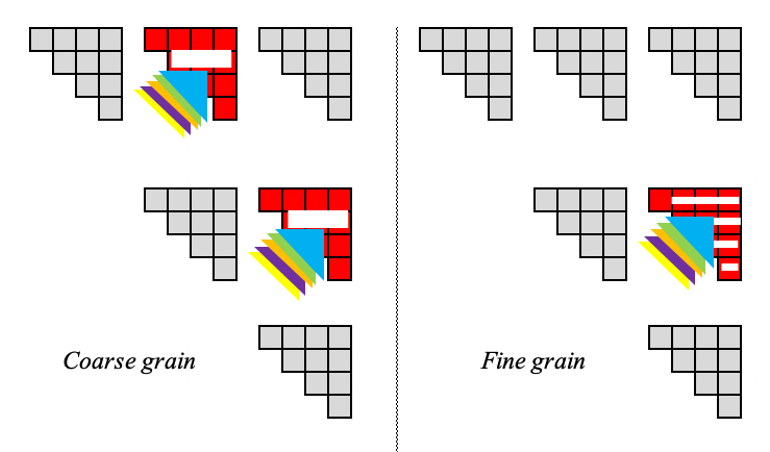
\includegraphics[scale=0.69,trim=5 5 5 5,clip]{content/figures/bpm_phase_2_memory_map.png}}
\caption{BPMax memory map without optimization}
\label{fig:bpm_phase_2_memory_map}
\end{figure}
Fine-grain requires only a $2-D$ array for each of the reduction variables illustrated in Figure~\ref{fig:bpm_phase_2_memory_map}. 
We almost eliminate the need for extra memory usage for the reduction variables using memory map transformations. $R_{0}$, $R_{3}$, and $R_{4}$ are always computed before the final $F$-table update in all of our schedules,
\begin{figure}[htbp]
\centerline{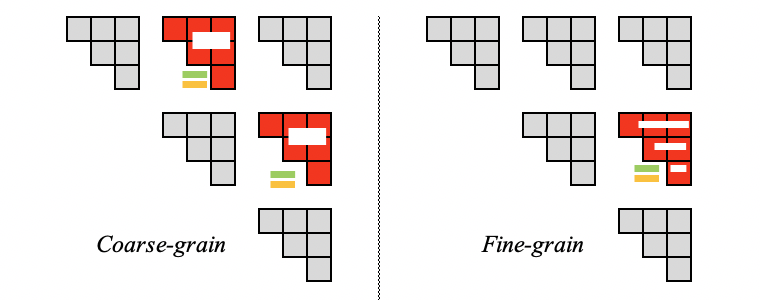
\includegraphics[scale=0.70, trim=5 5 5 5,clip]{content/figures/bpm_phase_3_memory_map.png}}
\caption{BPMax optimized memory map}
\label{fig:bpm_phase_3_memory_map}
\end{figure}
So, we use memory map transformations for $R_{0}$, $R_{3}$ and $R_{4}$ to share the memory with $F$-table. For the inner reductions - $R_{1}$ and $R_{2}$, our schedules update the final $F$-table entry bottom-up and then left to right where $j_{2}$ is the innermost loop. So, it accumulates intermediate results along a row. Thus, only one row of an inner triangle is required for $R_{1}$ and $R_{2}$ to keep up with the $F$-table update highlighted in Figure ~\ref{fig:bpm_phase_3_memory_map}.  Also, invocation of the subsystem calls creates new variables and copies data around by default. We optimize these redundant data copies using subsystem-related memory transformation.

\subsubsection{Performance Tuning}
We have attempted tuning various parameters such as tile size, OMP schedule, and memory maps to improve the performance. To find an optimum tile size, we started with cubic tiles and then adjusted the size of one or more dimensions to find a  tile size that works moderately well across various inputs. However,  we noticed that rectangular tiles work better than cubic tiles. 
\begin{figure}[htbp]
\centerline{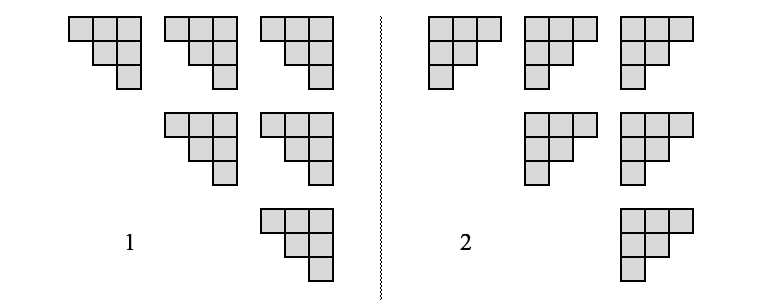
\includegraphics[scale=0.70, trim=5 5 5 5,clip]{content/figures/memory_map_update.png}}
\caption{Memory mapping schemes}
\label{fig:memory_map_schemes}
\end{figure}
We experimented the effect of OMP static, dynamic, and guided schedule and found that the OMP dynamic-schedule works better than the static and guided-schedule due to an imbalanced workload. We also performed some manual memory optimizations.  Scheduling transformation initializes memory for each reduction body (corresponding to a variable), but when one variable shares memory space with multiple variables,  memory initialization becomes redundant. The current code generator does not optimize it. We comment out these macros, which attempt duplicate initialization to eliminate redundancies. We have tried two different memory transformations for the inner triangles highlighted in  Figure~\ref{fig:memory_map_schemes} - 1 : $(i_{2}, j_{2} \mapsto i_{2}, j_{2})$ and 2 : $(i_{2}, j_{2} \mapsto i_{2}, j_{2}-i_{2})$ and found that the option-1 always performs better.

\subsubsection{Validation of Program Correctness}
In addition to checking the final scores between reference and optimized version, we use \alphaz\ toolset to verify the correctness of the optimized program using a verifier that compares the outputs of a schedule code with the sequential code. However, this is not sufficient due to the max-plus operation. We have developed a parallel version of the BPMax program to replace the max-plus with the plus-plus operation and apply the same sequence of transformations and run it through the verifier to ensure that our transformations and schedules do not change the semantics of the original program. One major challenge was running the validation on the longer sequences since the base, and sequential implementations are extremely slow.